\chapter{Development}

\section{Game design}

\subsection{Game concept}
\textit{Micorrizas} is based on the educational activity carried out in the \textit{Jardín de los Sentidos} as part of the subject related to the natural environment in Early Childhood Education. In this activity, students separated in groups visit the garden and work directly with the natural space through observation, identification and interpretation tasks. The aim is for students to understand the educational potential of nearby natural environments and to learn about the biodiversity of the garden through direct interaction with plants, sensory areas and ecological elements.

Since the original activity takes place outdoors and requires students to move through the different areas of the garden, \textit{Micorrizas} was designed as a mobile and geolocated experience. The mobile device makes it possible to guide the students through the physical space, detect their position and activate missions when the group reaches specific areas. In this way, the game preserves the relationship with the real environment while adding a digital layer of interaction, narrative progression and feedback.

The content of the game is organised through missions linked to the senses represented in the garden. Each quest focuses on a specific type of perception or knowledge: visual recognition of plants, identification of sounds, deduction of species from tactile characteristics, the relationship between fruits and species, and classification of plants according to their uses. The design of each quest was defined by combining the educational purpose of the original activity by each area of the garden (i.e.,...) with interaction models suitable for mobile devices. This type of interaction is detailed in Section \ref{sec:mechanics}.

Cooperation plays a central role in the design. Quests are completed as a group and the score obtained belongs to all members in the same game. Some quests rely on discussion and collective memory, while others distribute information across devices to encourage communication between players. This cooperative gameplay makes collaboration an active part of how the game functions and reflects the social nature of the original learning activity.

Main character’s narrative and the mycorrhizal network give unity to the experience. Each mission represents the recovery of a part of the garden and contributes to rebuilding the lost connection between the sensory zones. The game’s progression is presented as a symbolic restoration of the natural environment, linking players’ actions to the observation, interpretation and care of biodiversity.

% Imagen del mapa zonas definidas



%TODO ESTO MEJOR AÑADIR UNA SUBSECCIÓN DESPUÉS DE MECHANICS (CREO) QUE SEA DESIGN DECISION DUE TO PEDAGOGIAL AIM (HAY QUE DARLE UNA VUELTA) Y PONER TODO ESTO PORQUE NO LLEGA A SER GAME CONCEPT SOLO, SÍ DECISIONES DE DISEÑO PERO TENIENDO EN CUENTA QUE ANTES HAS EXPLICADO LAS MECÁNICAS

 This type of interactions was are simple, fast and well suited to mobile play. The binary gesture reduces interface complexity and allows players to focus on the recognition task. Since only one stimulus is presented at a time, the player’s attention remains centred on the plant profile and on the comparison with the real garden. The mechanic also supports short classification rounds, making the activity easy to understand and suitable for outdoor use. 
From a pedagogical perspective, the Sight quest reinforces visual discrimination. Players must classify each species by comparing visual evidence, their memory of the physical route and the information shown on the card. The simplicity of the interaction allows the challenge to remain focused on observation and decision-making, while the immediate feedback helps players correct mistakes and progressively refine their understanding of the plants present in the garden.

The Sound mission was designed to connect auditory perception with cooperative interaction. Its structure was inspired by two types of activities: audio-based association exercises, such as Duolingo, and collaborative answer distribution, similar to the dynamic used in Quizlet Live. In each round, one device plays an audio clue related to a sound found in the garden, while the rest of the devices display different possible answers.

Only one of the devices contains the correct answer, so the group must communicate in order to identify it. Players need to listen to the sound, compare the available options and decide together which response should be selected. Once the group answers (correctly or incorrectly), the roles change: another device becomes responsible for playing the sound, while the previous audio device receives answer options. This rotation ensures that the task is distributed among the participants and that all players take part in both listening and decision-making.

From an educational point of view, this mission works on sound recognition, association and group communication. The audio clue connects the digital interaction with the sensory experience of the garden, while the distribution of answers across devices encourages players to share information and coordinate their response. As a result, the mission transforms a simple sound-identification task into a cooperative activity linked to the physical environment.


\subsection{Lore}
Deeproot (see Figure \ref{fig:Deeproot}) is the main character in \textit{Micorrizas}  and acts as the game’s narrative guide. He is an Ent, a creature directly linked to the flora of the \textit{Jardín de los Sentidos}, whose role is to protect and manage the area’s natural resources. Due to the slowness inherent to his species and the progressive deterioration of the garden, Deeproot seeks the help of a group of adventurers, represented by the players, to restore the lost balance.
\begin{figure}[htpb]
    \centering
    
\includegraphics[width=0.3\textwidth]{img/Deeproot.png}
    \caption{Deeproot the main character}
    \label{fig:Deeproot}
\end{figure}

The story begins with a conflict caused by the negligence of the human race. For a long time, natural spaces and their biodiversity have been polluted, ignored and displaced, weakening the relationship between people and the environment. In the past, nature flourished throughout the university’s grounds, and the \textit{Jardín de los Sentidos} occupied a central place within that ecosystem. It was the heart of all the flora in the realm and maintained a connection with the rest of the green spaces via an underground network formed by conduits covering the plants’ roots, as can be seen in Figure \ref{fig:mycorrhizae}.

\vspace{0.5cm}
\begin{figure}[htpb]
    \centering
    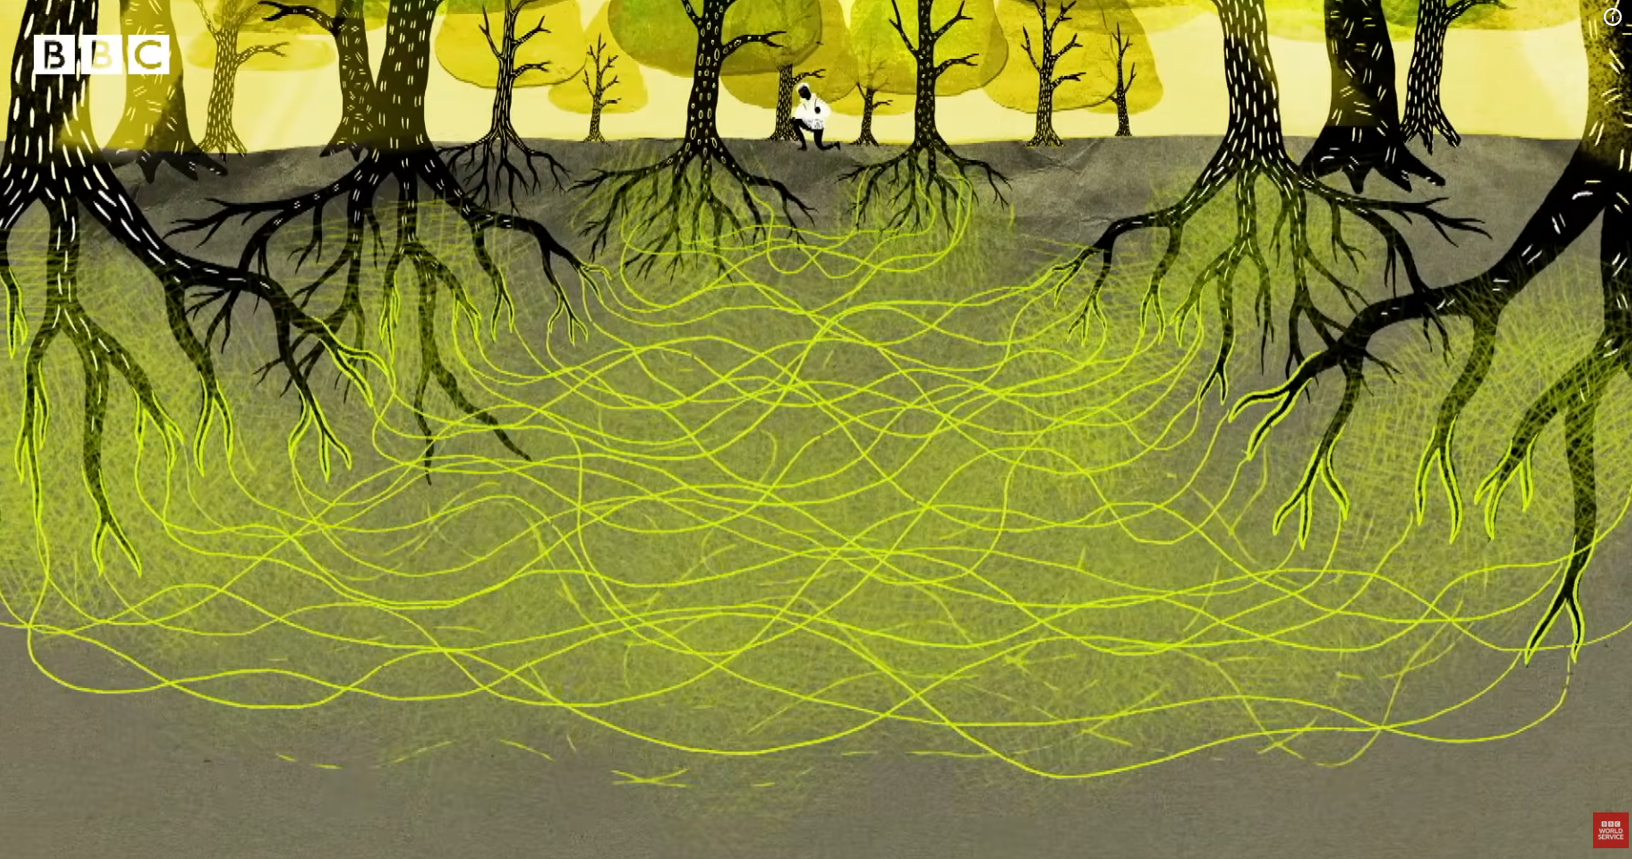
\includegraphics[width=\textwidth]{img/Micorrizas.png}
    \caption{Mycorrhizae by BBC World Service\protect\footnotemark}
    \label{fig:mycorrhizae}
\end{figure}

\footnotetext{Resource: BBC World Service \cite{BBCWorldService}.}

These conduits were made up of mycorrhizae, the symbiotic relationship between a fungus’s mycelium and a plant’s roots, and enabled the \textit{Jardín de los Sentidos} to send nutrients, signals and information to the rest of the flora. Thanks to this network, the plants were able to remain connected, and the garden functioned as a living organism capable of perceiving, remembering and transmitting knowledge through its senses.

At present, this network is fragmented and weakened. The garden’s senses have lost part of their memory, and Deeproot can no longer transmit information correctly via the mycorrhizae. Even so, the network can still be restored. To achieve this, players must explore the \textit{Jardín de los Sentidos}, complete the various missions associated with each sensory zone, and help restore the lost connections.

Once the group has managed to restore the garden’s senses, Deeproot will once again be able to channel information through the mycorrhizal network. The restoration of this connection symbolises the recovery of the bond between humans and the natural environment, as well as the ability to observe, understand and appreciate the biodiversity that forms part of the garden.


\subsection{Game Loop}
The game loop in \textit{Micorrizas} is structured around the physical exploration of the \textit{Jardín de los Sentidos} and the triggering of quests via geolocation. The experience begins on the connection screen, where one player creates the game as the host and the other participants join using a code. Once the session has been established, all players access the map scene, which serves as the central hub for navigation and group coordination.

Upon entering the map scene, the system checks the players’ positions. If the group is outside the \textit{Jardín de los Sentidos}, Deeproot appears to indicate that assistance can only begin once everyone has arrived at the garden. This initial condition links the start of the game to physical presence in the space and reinforces the geolocation-based nature of the experience.

Once all players are within the playable area, Deeproot introduces the main objective: to explore the garden and find the missions needed to repair the mycorrhizal network. From this point onwards, the group can move freely around the map. Progression follows a non-linear structure, as the five missions associated with the senses can be completed in any order. This decision allows the journey to adapt to the group’s actual movement through the garden and avoids imposing a rigid sequence on the physical space.

The main loop is repeated in each sensory zone. Players explore the environment, enter a mission’s activation area, receive the corresponding narrative context, solve the mission cooperatively, and receive feedback on their result. Upon completing the mission, the system records the group’s score, marks that zone as completed, and returns the group to the map to continue their exploration. The group of adventurers can only complete each mission once. However, they can replay the entire game to achieve a higher score, as if they score less than 5, they will not have succeeded in restoring the mycorrhizal network.

Once all five missions have been completed, the game proceeds to the final screen. This scene displays the group’s name, the participants’ names and the group score achieved during the session. Deeproot concludes the experience by thanking the players for their help and explaining that the mycorrhizal network has restored its connections. This conclusion serves a dual purpose: it summarises the team’s results and provides a narrative conclusion to the journey through the garden. These results can then be used by the course lecturers to mark the activity on which the project is based.

\begin{figure}[htpb]
    \centering
    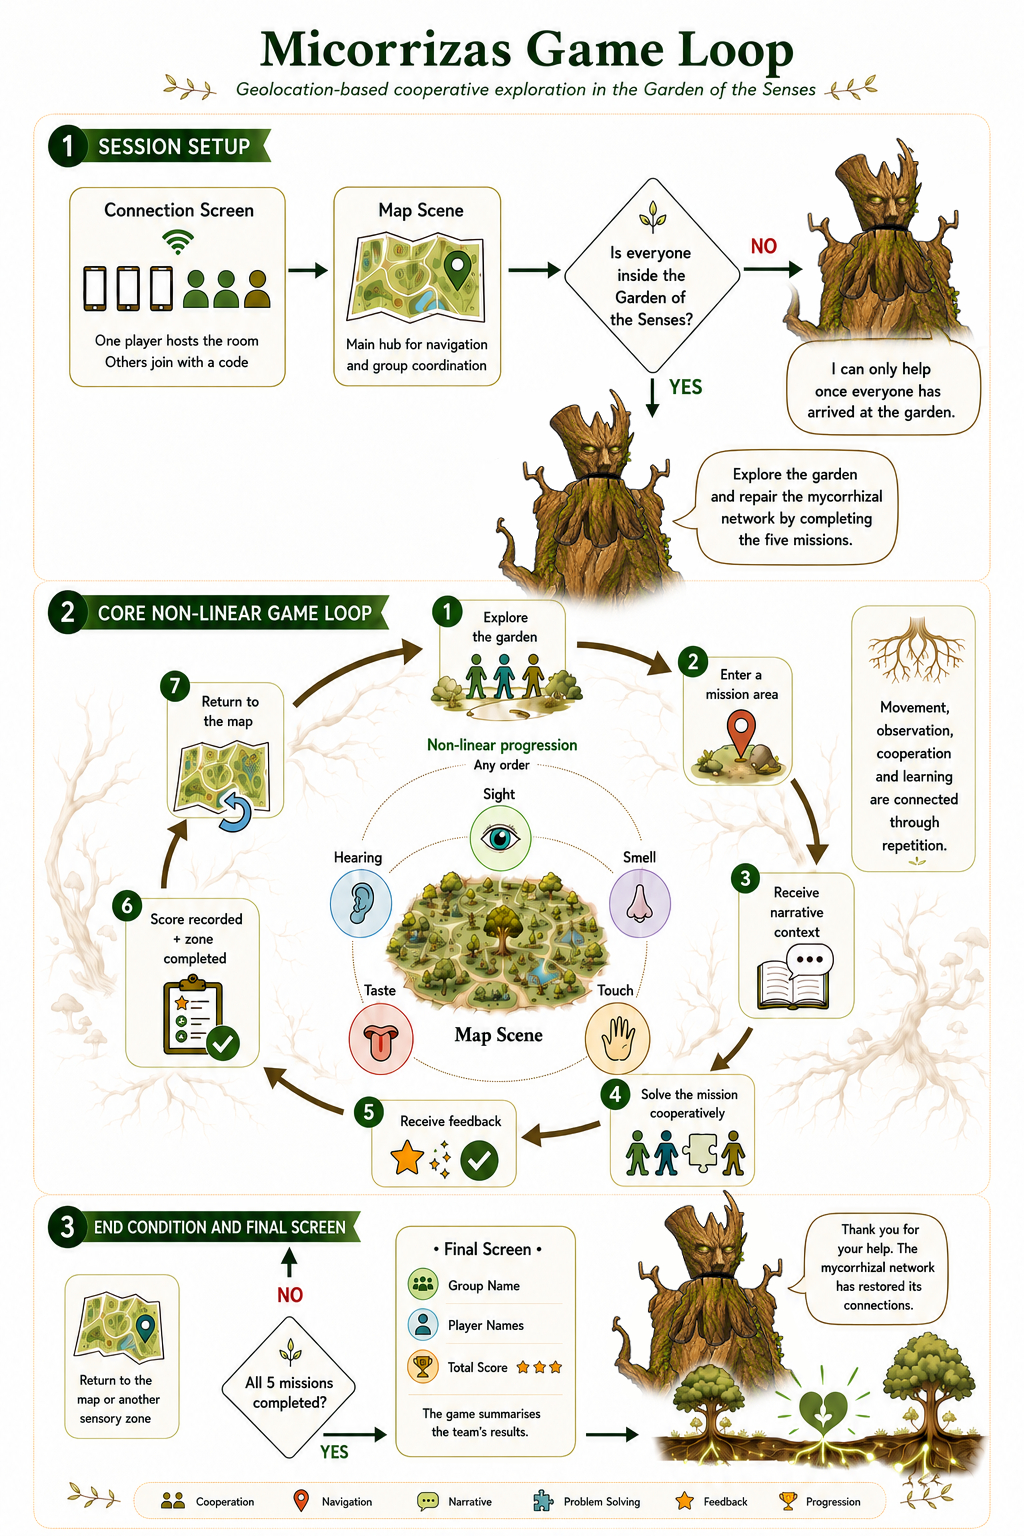
\includegraphics[width=0.9\textwidth]{img/MicorrizasGameLoop.jpg}
    \caption{Micorrizas game loop}
    \label{fig:gameloop}
\end{figure}


\subsection{Scenes from the game}
The \textit{Micorrizas} experience is organised into several scenes that structure the player’s journey from the creation of the session to the end of the game. Each scene fulfils a specific function within the overall flow and helps to distinguish the different phases of the game: connecting the group, exploring the garden, completing missions, and presenting the final result.

The first scene corresponds to the lobby system. Here, one player creates the room as host and the other participants join using a code. This scene allows the group to form before the experience begins and ensures that all players enter the same cooperative session.

Once connected, players access the map scene. This scene represents the \textit{Jardín de los Sentidos} through the integration of ArcGIS and shows the players’ positions within the physical space. The map serves as the navigation hub of the experience, as it is from here that the sensory zones are detected and the corresponding missions are activated. It also allows the group to check which zones they have completed and which remain to be explored.

The mission scenes constitute the main playable part. They all share a common structure: a header at the top displays the mission objective, the relevant score or progress, and the necessary instructions so that the group knows what to do at all times. Missions are carried out cooperatively and the result obtained belongs to all members in the same room. At the end of each mission, the group receives a score between 0 and 10, which is added to the game’s overall progress.

Each sensory garden has its own mission. In the Garden of Sight, players practise visual recognition of plant species using plant cards featuring an image and scientific name. In the Garden of Hearing, the group listens to sounds related to the environment and must identify them with the help of a distorted black-and-white visual clue. In the Garden of Touch, players deduce a plant from progressive clues related to physical and sensory characteristics. In the Garden of Taste, the mission uses a memory game played in pairs, themed around plants and fruits from the garden. In the Garden of Smell, players classify plants using a drag-and-drop interaction, linking them to areas such as decorative, culinary or medicinal uses.

The final scene corresponds to the final result. This screen appears when the group has completed the five main missions. It displays the group’s name, the names of the participants and the group score achieved. Deeproot reappears to narratively conclude the experience and thank the players for their help in restoring the mycorrhizal network.


\subsection{Game Mechanics}
\label{sec:mechanics}
The game mechanics of \textit{Micorrizas} are organised into two levels: a core mechanic common to the entire experience, and a set of specific game mechanics associated with each mission. 

The core game mechanic is the physical exploration of the \textit{Jardín de los Sentidos}. Players advance by moving through the real space, and the system uses geolocation to detect when the group enters a sensory zone. Upon reaching one of these areas, the corresponding mission is triggered and the player’s action shifts from the map to the challenge scene.

This main game mechanic allows movement through the garden to form part of the gameplay itself. Players use the map to orient themselves, locate pending zones and check the group’s progress. Geolocation links the participants’ real-world position to the narrative and gameplay progression, so that each mission is tied to a specific location within the environment.

All missions share several cross-cutting mechanics. The first is cooperation, as challenges are solved as a group and the score belongs to all players in the same room. The second is immediate feedback, which informs the group of the result obtained upon completing each mission. The third is shared progression, which records the areas completed and allows the group to move towards the conclusion of the experience. These mechanics maintain the game’s coherence even though each mission uses a different form of interaction.

The specific game mechanics associated with each mission are described below.

\textbf{Garden of Sight}
In the Garden of Sight, the mission uses a card-swiping mechanic. In each round, a card appears showing an image of a plant and its scientific name. Players must decide whether that species has been observed in the Jardín de la Vista. To answer, they swipe the card to the right if they believe it belongs in that area, and to the left if they believe it does not. This interaction is well suited to mobile devices because it is quick, straightforward and easy to understand. The mission develops visual discrimination, as players must compare the information on the card with what they remember having observed in the real environment.

\textbf{Garden of Hearing}
In the Garden of Hearing, the mission combines sound identification and cross-device cooperation. One player plays an audio clip related to the garden and the other devices display possible answers. The correct answer appears on only one of the mobiles, so the group must communicate to locate and select it. The mechanics draw on exercises involving the association of sound and word, alongside a distribution of answers among participants to reinforce collaboration. After each round, the device responsible for the audio changes, allowing different players to take on different roles during the mission.

\textbf{Garden of Touch}
In the Garden of Touch, the mission is based on a progressive deduction mechanic. Players must write the name of a plant that might be found in that area of the garden. Each attempt generates a visual response showing partial information about the proposed species. Initially, the system reveals general characteristics, such as roughness or shape. As new attempts are made, more specific clues are unlocked, such as characteristics of the fruit, type of leaf or type of plant. This mechanic encourages comparison, the elimination of possibilities and discussion among players.

\textbf{Garden of Taste}
In the Garden of Taste, the mission uses a memory-matching mechanic. Each device displays several face-down cards relating to fruits or plants in the garden. Players can reveal cards on their own devices, but pairs are never complete on a single mobile. To solve the mission, the group must communicate which cards each participant has discovered and coordinate to find the correct matches. This structure transforms a classic memory game into a cooperative activity distributed across devices.

\textbf{Garden of Smell}
In the Garden of Smell, the mission uses a drag-and-drop mechanic. Players receive plant cards and must sort them into categories related to their use or function, such as decorative, culinary or medicinal. The interaction involves dragging each card to the corresponding section. This mechanic allows players to practise associating plant species with human uses, whilst maintaining an interaction that is clear and accessible on mobile devices.

\subsection{Porque de las desionsiones}


\subsection{Game art}
The visual design of \textit{Micorrizas} was created to support the educational and environmental tone of the project. Since the game takes place in the \textit{Jardín de los Sentidos} and focuses on biodiversity, the art direction is based on a natural and friendly aesthetic. The predominant colour is green, which evokes vegetation, nature and ecological restoration. This is combined with brown and earthy tones, especially in elements related to Deeproot, trees, roots and the mycorrhizal network.

The game combines two visual approaches. On the one hand, the map has a more realistic function, as it represents the real physical space where the players move. Its purpose is to help players understand their position in the garden and connect the digital experience with the actual environment. On the other hand, the character, interface elements and icons use a simpler and cleaner style, based on flat colours, clear shapes and readable visual elements. This contrast allows the map to preserve its connection with the real location while the interface remains accessible and easy to understand on a mobile screen.

The interface was designed to be simple and direct, as the game is intended to be played outdoors. Players need to understand the information quickly while walking through the garden and interacting with the rest of the group. 

Deeproot is the most important character in the visual identity of the game. His design had to communicate his connection with nature, age and wisdom, while also making him approachable as a guide for the players. The Ent’s silhouette was created using Illustrator as a vector drawing, whilst the final texturing was carried out with the help of AI to achieve a bark-like appearance, complete with moss and natural details. This process resulted in a character that fits within the game’s fantasy narrative, whilst maintaining a visual connection with the garden and its vegetation.

The missions also required specific visual resources. Some assets were created or adapted for the project, while others were selected from external asset libraries such as the Unity Asset Store and Itch.io. In the Garden of Hearing mission, the images used as visual clues were processed with filters so that they would not reveal the answer too directly.

Audio resources were also part of the artistic and sensory design of the game. Since the Garden of Hearing mission is based on recognising sounds related to the natural environment, sound selection was especially important. For this purpose, specialised sound databases such as Xeno-canto were used to search for accurate recordings. The selected sounds were recordings made in Spain, so that the audio material would remain coherent with the geographical and environmental context of the project.


\section{Tecnical Architecture}
The project’s architecture is organised into four main blocks: connection and cooperative session, geolocation, spatial representation in ArcGIS, and the cooperative mission layer. Each block has a specific responsibility and communicates with the others via events, synchronised state structures and scene transitions, as can be seen in Figure \ref{fig:architecture}.

The architecture can be described as a combination of several layers, each with a specific responsibility within the game’s overall operation.

Firstly, there is a bootstrap and network connectivity layer, responsible for launching the application and enabling players to create a co-operative session or join an existing one. This layer establishes the connection between devices before the game begins.

Above this lies the session layer, which maintains the game’s shared global state. In other words, this layer ensures that all players are working with the same information: which mission is active, what stage the game is at, or which elements have been completed.

The geolocation layer retrieves the device’s actual position via GPS and converts it into information useful for the game. In this way, the player’s physical location can be synchronised with the other participants and utilised within the co-operative experience.

Next, the map and spatial interaction layer transforms the geographical coordinates into visible and interactive elements within the game, such as markers, trigger zones or points of interest. Thanks to this layer, the real-world space of the \textit{Jardín de los Sentidos} becomes part of the playable world.

Finally, the mission layer organises the game’s activities. This layer is built on a common foundation that allows the general flow of missions to be reused, their results to be managed, and the transition between their different phases to be controlled.

On a practical level, this architecture relies on tools such as Unity Relay, to facilitate connections between players; Netcode for GameObjects, to synchronise information between devices; and the ArcGIS Maps SDK, to work with maps and geographical coordinates. In addition, proprietary services and drivers have been developed to clearly separate data collection, synchronisation, visual representation and the user interface.

\begin{figure}[htpb]
    \centering
    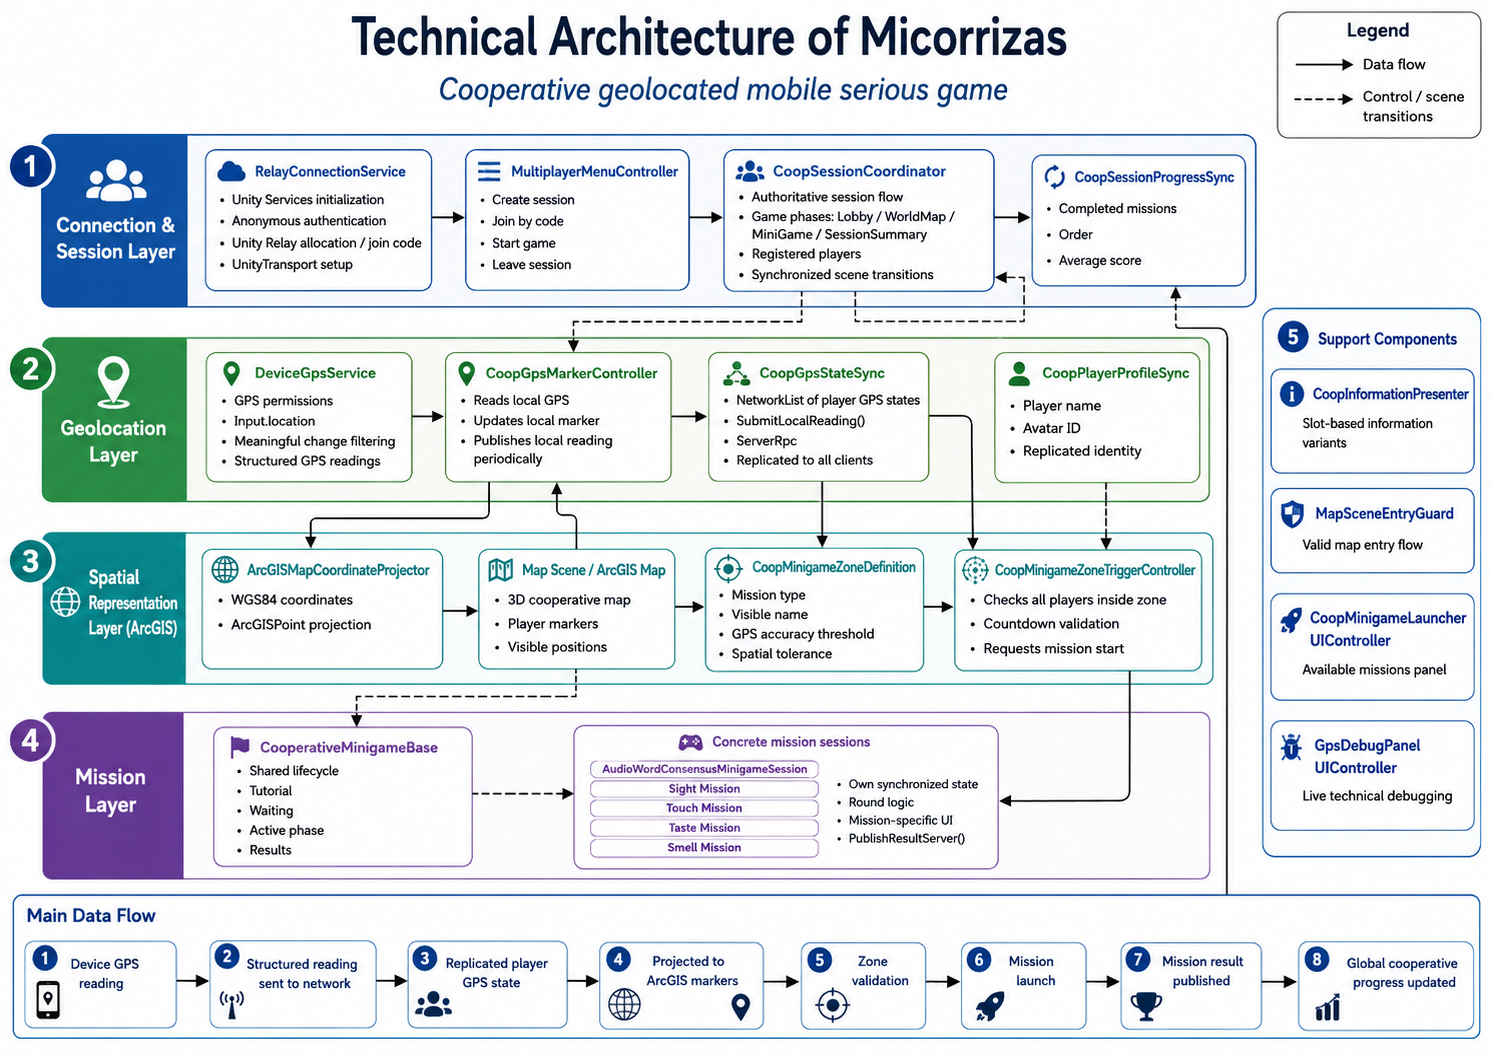
\includegraphics[width=0.9\textwidth]{img/Architecture.png}
    \caption{Micorrizas Architecture}
    \label{fig:architecture}
\end{figure}



\section{Problems and solutions}
% Igual aqui podria hablar de lo del cambio de proyecto de HDRP a URP 
During development, the main difficulties were related to geolocation, mobile testing and the integration of several technical systems into a single gameplay flow.

The first major challenge was the implementation and testing of geolocation. As the game relies on the player’s position in a real-world outdoor environment, the system could not be fully validated within the Unity editor. The location service had to be tested on a real Android device, which slowed down the process and made it less predictable. To address this issue, the geolocation system was developed incrementally: first by loading and centring the map, then by limiting the rendered area, and finally by adding trigger zones for each sensory garden. The trigger zones were designed with generous radii to compensate for GPS inaccuracies.

The multiplayer system also required several design and technical decisions. The project required cross-device cooperation, but the gameplay did not require real-time character movement or complex online interaction. For this reason, the multiplayer implementation was limited to session creation, access codes, player connection, synchronisation of shared states, and group scoring. This reduced the system’s complexity whilst preserving the game’s cooperative structure.

A final challenge was integrating the mini-games with the rest of the application. Each mission had its own interaction model, but they all had to share the same session structure, scoring logic and progression system, so that it could be reused. To resolve this, the mini-games were connected to a common flow: activation from the map, execution of the challenge, calculation of the group score and return to the main progression.

\section{Deviations from the initial proposal}
The initial proposal was based on creating an escape room or gymkhana inspired by the activity suggested by the Early Childhood Education teachers. This first approach aimed to transform the guided visit into a sequence of challenges distributed throughout the \textit{Jardín de los Sentidos}, using the physical space as the basis for the player’s progression.

After an initial brainstorming process with the project supervisor, the escape room structure was reconsidered. The project started to move towards a mixed reality experience in which users could learn about the biodiversity of the garden through digital information layered over the physical environment. This direction was interesting from a design perspective, since it allowed the real garden to remain central while adding interactive digital content connected to its plants, sensory areas and educational value.

However, after discussing the proposal with the Early Childhood Education teachers, the mixed reality approach was identified as difficult to apply in a realistic educational context. The main limitation was the accessibility of the required technology. A mixed reality experience would depend on specific devices that are not commonly available to students or teachers, making it harder to use the project as a practical tool during the real activity.

For this reason, the project was refocused on mobile devices, whilst ensuring that the main focus of the project remained the biodiversity of the \textit{Jardín de los Sentidos}. This decision made the game more accessible and better suited for use directly in the garden, given that most potential users already own a mobile phone. The mobile platform allowed the project to maintain a connection with the physical space whilst reducing the technological barriers to the experience. From that point onwards, the design focused on developing a game for Android mobiles that could combine geolocation, cooperative interaction and educational quests within the \textit{Jardín de los Sentidos}.

